\documentclass[man,noapacite]{apa2} 

\usepackage{url}
\usepackage{apacite2}
\usepackage{amssymb}
\usepackage{graphicx}

\title{Using Tablets to Collect Data from Young Children} 

\author{Michael C. Frank, Elise Sugarman, Alexandra C. Horowitz, \\ Molly L. Lewis, \& Daniel Yurovsky} 
% \author{~}
% \affiliation{~}
\affiliation{Department of Psychology, Stanford University}

\abstract{Mobile, touch-screen devices are increasingly ubiquitous in children's lives. The extensive use of such devices presents an exciting opportunity for data collection. We describe a simple method for creating cross-platform, interactive tablet experiments using open web-based resources. We illustrate this method by collecting data from one- to four-year-old children in a word-recognition paradigm, using three different techniques: tablets, eye-tracking, and an in-person storybook paradigm. Both accuracy and reaction time data from the tablet compared favorably to the other methods. Tablets should be considered as a viable method for collecting low-cost, well-controlled developmental data.}

\shorttitle{Tablet-Based Data Collection} 
\rightheader{TABLET-BASED DATA COLLECTION}

\acknowledgements{This work supported by a John Merck Scholars award to MCF. We gratefully acknowledge the families and staff at Children's Discovery Museum of San Jose and the laboratory of Anne Fernald for sharing their visual stimuli. An earlier version of this material was previously presented in a blogpost \cite{frankblogpost}. Thanks to Janelle Klaas, Andrew Weaver, and Sarah James for assistance in data collection. Please address all correspondence to Michael C. Frank, Department of Psychology, Jordan Hall (Bldg. 420), 450 Serra Mall, Stanford, CA 94305. Phone: (650) 724-4003. E-mail: \texttt{mcfrank@stanford.edu}}

\begin{document}

\maketitle


\section{Introduction}

Since Apple debuted the iPad in 2010, the ubiquity of personal tablets---interactive, touchscreen-based computing devices that are typically larger than a phone but smaller than a laptop---has skyrocketed. By 2014, an estimated 71\% of families with young children in the United States owned a ``smart'' mobile device, with 55\% of households owning tablets (27\% of lower-income families and 63\% of higher-income families); tablets were estimated to constitute 13\% of children's overall screen time from ages 0--8 \cite{rideout2014}. Accordingly, the market for downloadable applications targeted for children has increased dramatically. In one estimate, applications targeted towards children were 72\% of the top selling items in the iTunes store, and over 80\% in the Education category \cite{shuler2012}. The explosion in popularity of touchscreen devices has created a surge of interest in the potential for using these devices as scientific tools. 

Unlike in the case of traditional behavioral experiments and eye-tracking measures, there are relatively few resources to help labs implement tablet experiments. In addition, the reliability of data gathered from tablet experiments from young children has not been tested. The goal of the current article is to address these challenges. We begin by briefly reviewing research on the use of tablets with children. We then describe a method for creating tablet-based experiments using standard, freely-available web-development tools. Although this method requires some programming experience, it is significantly easier than developing tablet-native applications (e.g., apps that can be downloaded from the Apple App Store or Google Play platforms and are specific to a particular device). We report data on an experiment comparing word-recognition accuracy and reaction time across tablet, eye-tracking, and behavioral data collection. Our findings suggest that the tablet platform is an engaging method for data collection that, when used appropriately, can yield reliable estimates of accuracy and reaction time from young children. 

%Nevertheless, there are significant challenges involved in using tablets for research, especially for preschool children. These include the difficulty and potential costliness of developing custom applications (``apps'') for individual experiments, and technical problems with app distribution and cross-device compatibility. In addition---although some experimental tasks have been administered using touch screen computers and some standardized tasks have been ported to tablets---there is a little data confirming the reliability of tablets as a platform for data collection with children. Perhaps for these reasons, few published articles have used tablets to collect developmental data. 
%

\section{Prior Work on Using Tablets with Children}

Although tablets are becoming increasingly common in research, relatively little published work has compared them directly with other data collection modalities. One exception to this statement, however, is the use of tablets in standardized psychological instruments. Publishers are increasingly creating tablet-specific versions of paper-and-pencil assessments; at time of writing, a number of instruments---including the WAIS \cite{wechsler2008}, CELF \cite{wiig2004}, PPVT \cite{dunn2007}, and many others----are available from commercial publishers. The tablet modality assists in standardizing instructions and facilitates response logging, both with minimal changes to the basic instrument. Thus, it seems clear that tablets can be used effectively for data collection with preschool-aged and older children in relatively straightforward and standardized paradigms. 

For younger children, the primary focus of research on tablets has not been on their use as a data-collection platform but rather the evaluation of their educational potential. The starting point for investigations of learning from tablets is the suggestion that children learn less from passive video viewing than they do from live demonstrations, a phenomenon known as the ``video deficit'' effect \cite<e.g.>{anderson2005,deloache2010}. The experiences offered by touch-screen devices may be distinct from passive viewing of television and computer screens, however. For example, \citeA{zack2009} found that 15-month-olds were able to transfer knowledge about an object learned via a touch-screen to a physical toy. Practice with interactive games may also benefit attention and motor control \cite{bavelier2010}, and more generally screen time with tablets can promote independence, opportunities for physical closeness, and feelings of fun and accomplishment \cite{rvachew2013}. The contingent feedback and individualization offered by mobile devices may thus make them a better medium for learning and engagement than traditional view-only screens, and these advantages may also increase their utility for data-acquisition.

The accuracy of young children's motor control poses a concern about their performance using tablets. Experience likely plays a substantial role in modulating the accuracy of tablet interactions, especially for the toddlers and early preschoolers, and some gestures are easier than others. \citeA{aziz2014} tested 2- to 5-year-olds in Malaysia and the United Kingdom on their ability to perform the seven most common touch gestures of iPads: tap, drag/slide, free rotate, drag and drop, pinch, spread, and flick. By age 2, children mastered the tap and drag/slide gestures, and by age 3, they could reliably produce all but the spread gesture. By age 4, all children performed all of the gestures. Our experiences confirm that even 1.5 -- 2-year-olds are able to learn to tap targets without too much difficulty, though more sophisticated gestures may be too complex for them. 

While relatively little published research has made use of novel tablet-based tasks, there is an extensive literature that has used lab-based touch screen paradigms with children \cite<e.g.>{friend2003,holloway2008, sage2015}. This prior literature is important for calibrating our expectations about what paradigms may be ported successfully to tablets, but if anything it is likely to underestimate the utility of tablets. Touch screen paradigms are often conducted with relatively specialized equipment in a lab setting, while tablets can be used anywhere. In addition, tablets are small enough to be held by the child, and generally require small motor movements; in contrast, touch screens are typically on a desk or mounted on a wall and may require a full arm movement (leading to fatigue over a longer testing session). Finally, the increasing comfort and proficiency of even young children with tablets may lead them to be more comfortable with experiments conducted in this medium, in turn resulting in better data.

% In sum, while tablet experiments for young children requires age-appropriate calibration of gesture and content complexity, they are an engaging and promising experimental modality. In the next section, we describe our experiences 

% In addition, more research is needed to understand how tablets compare with other data collection modalities. 

\section{Why Collect Developmental Data With Tablets?}

% \subsection{The value of tablet-based data collection}

Researchers working with young children have access to a wide variety of experimental paradigms, ranging from behavioral forced-choice to eye-tracking and looking time-based measures \cite{aslin2007,gredeback2009}. Each of these methods has its drawbacks. Behavioral methods are flexible and easy to implement, but they can be subject to experimenter biases, and often require labor-intensive offline coding. In contrast, corneal-reflection eye-tracking methods are precise and unbiased, allowing tight experimental control, but can be expensive and are difficult to implement outside of tightly-controlled lab settings. In addition, eye-tracking paradigms are typically very limited in length as they tend to be non-interactive \cite<cf.>{deligianni2011}, and often result in substantial data loss due to excessive movement, calibration issues, etc.

Tablet-based experimental paradigms can supplement both of these data collection modalities by allowing researchers to create engaging, interactive paradigms that are low cost but nevertheless offer some of the precision and experimental control of eye-tracking paradigms. In the sections below, we offer five reasons why tablets may be valuable tools for developmental research.

\subsubsection{Diverse measures} Tablets allow the collection of many different dependent variables, including forced-choice responding and gesture trajectories. We especially highlight the ability to measure reaction times using tablets. Reaction times provide a continuous, informative measure of cognitive process and have proven invaluable in both developmental \cite<e.g.>{fernald1998,marchman2008} and adult (e.g. \citeNP{sternberg1969} et seq.) studies. Behavioral paradigms that afford reaction time measurement for young children typically require time-consuming offline coding. In contrast, eye-tracking paradigms yield reaction times, but with the tradeoff that the paradigms themselves typically have limited interactivity. 

\subsubsection{Engagement} Children across a wide range of ages enjoy tablets and are highly motivated to explore new tablet-based tasks, allowing researchers to collect more data from individual children. As is obvious from infants' and young children's interest, these devices are extremely engaging  (for further evidence, see \citeNP{couse2010}). In addition, the use of tablet-based devices may lead children to view experiments as similar to desirable commercial apps. Behavioral paradigms with young children often require a ``warm-up'' period so that the child is comfortable interacting with an unfamiliar experimenter; such a period can be shorter or absent to the extent that a tablet-based paradigm requires less face-to-face interaction. 

\subsubsection{Experimental control} Studies that involve interaction with an experimenter are the de-facto standard in cognitive development research, but such studies have as major drawbacks that it may be difficult or impossible to ensure that experimenters are blind to condition and hypothesis. Often hypotheses are simple enough that even ``na\"ive'' research assistants can infer the experimental structure or the desired response. While there are methods for avoiding such issues, the possibility of eliminating experimenter bias via computerized stimulus presentation is attractive for situations where it is possible. And even when bias is not introduced, there are significant challenges in training a group of research assistants to implement an experimental protocol uniformly. Thus, tablet-based experiments can alleviate concerns about bias and uniformity of experimental presentation.

\subsubsection{Inclusion of special populations} Tablets can be a valuable tool for working with children who have learning or physical disabilities \cite<e.g.>{cardon2012, waddington2014, chai2014, bertucco2013}. The lack of face-to-face interaction demands make tablets especially appealing for working with children on the autism spectrum, who may find interactions with an unfamiliar experimenter especially aversive.

\subsubsection{Scale} Low cost and high accessibility make it possible to distribute tablets to research assistants who can collect data in a wider variety of locations (though not without concern about environmental distractions). In addition, it is in principle possible that children could contribute data to experimental studies via experiments administered by their parents or caregivers.
% \footnote{For an example of this method, see \url{http://lookit.mit.edu}, a web-based platform for looking-time experiments that engages parents as experimental confederates.} 
This latter possibility might be truly revolutionary in changing the scope of developmental data collection, though there are many challenges that such a data collection effort would need to overcome.

Despite all of these advantages, there are significant technical issues related to app creation that have slowed the adoption of tablet-based methods in developmental research (as well as other limitations, which we return to below). On the technical side, creating tablet-native apps---those that can be accessed through an Android or iOS tablet's main menu---requires substantial programming expertise. Worse yet, this expertise is not transferrable across tablet platforms. Developing a native app for iOS requires programming in Objective-C using Apple's proprietary app development tools; development for Android requires programming in a Java variant. In other words, either an investigator must learn a special-purpose programming language, or a programmer must be employed. This latter option is more common, but costs can easily run in the tens of thousands of dollars; in this sort of scenario, making scientifically-useful changes to an app may be undesirable because of added costs. 

\section{A Web-Based Method for Developing Tablet Experiments}


\begin{figure}[t] 
  \begin{center} 
    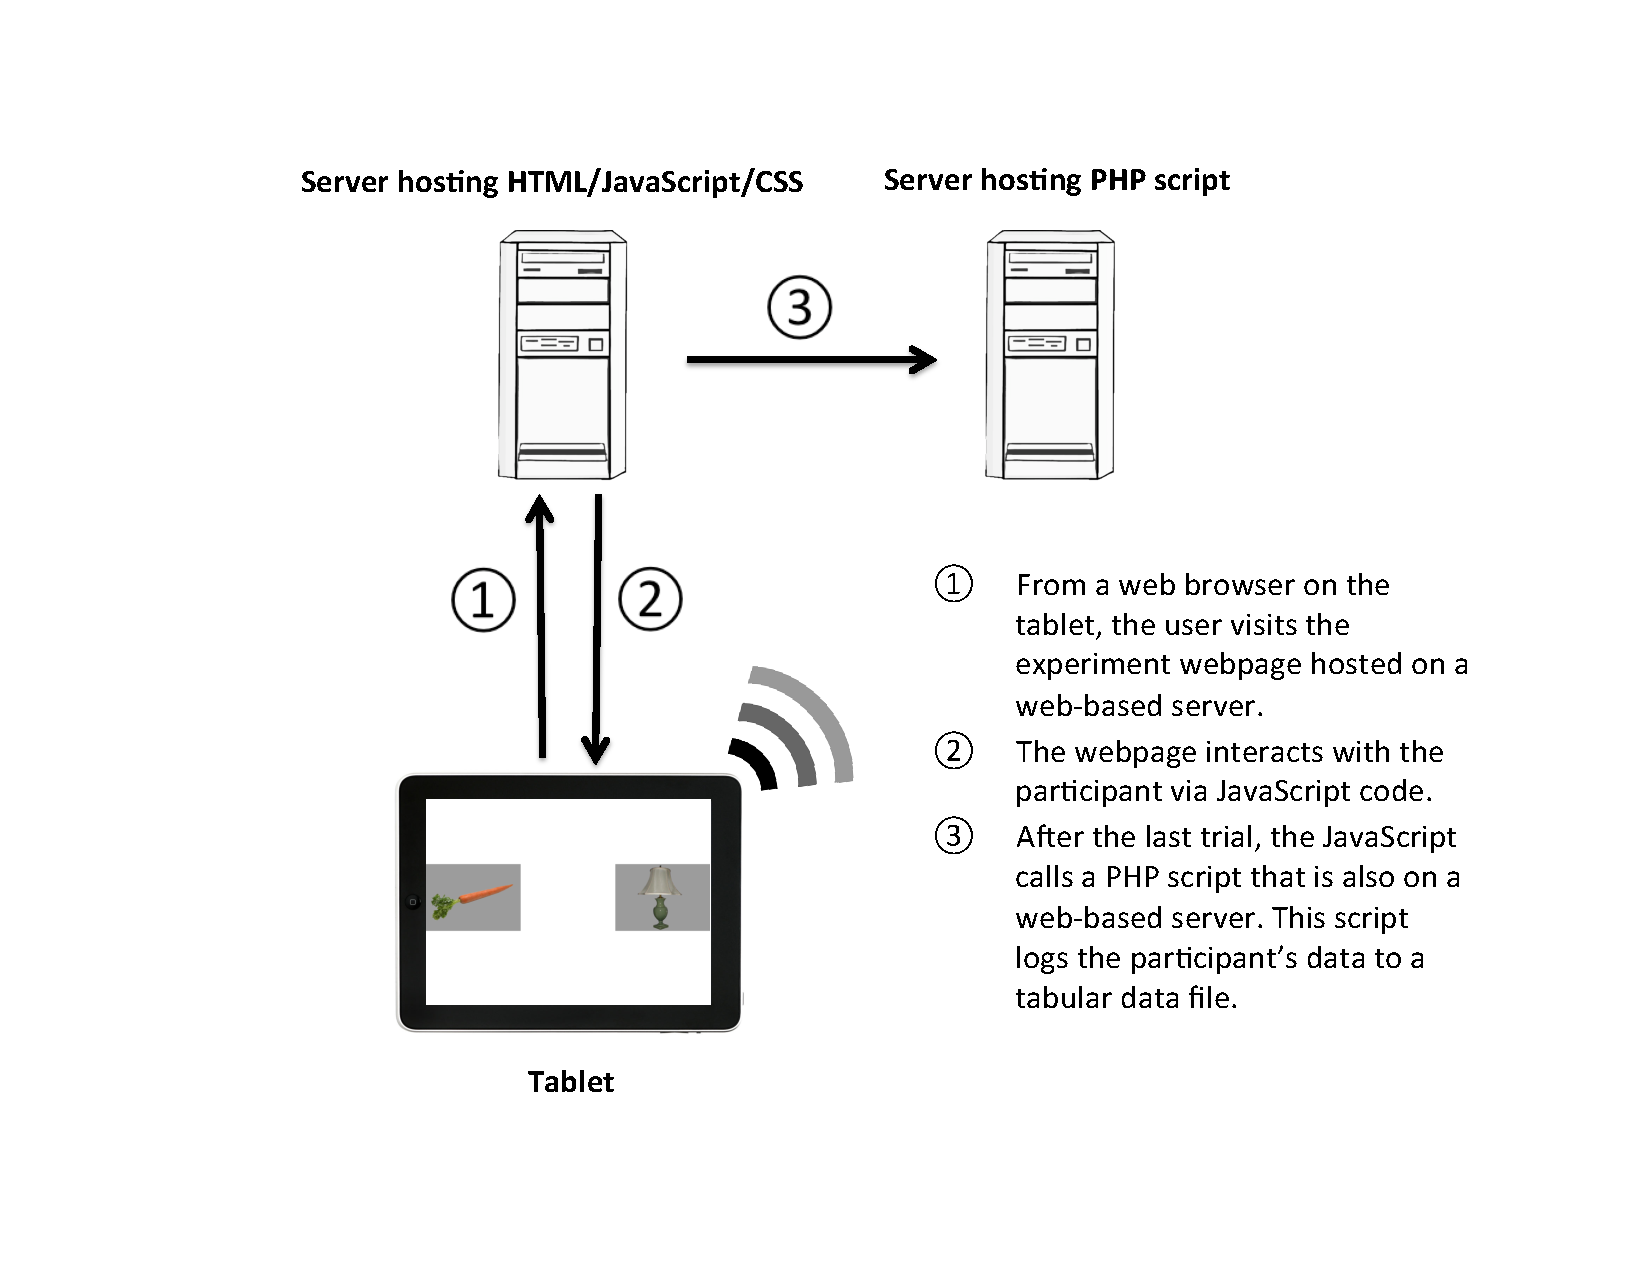
\includegraphics[width=4.5in]{figures/diagram.pdf} 
    \caption{\label{fig:diagram} A schematic of our method of collecting tablet data using a web-based experiment. Note that the two server functions can be executed by the same system; we have separated them here for clarity.}
  \end{center} 
\end{figure}

In contrast to costly, special-purpose methods, here we describe an alternative method for prototyping and collecting data on tablets. The method relies on creating the experiment as a simple webpage and then showing this page in the tablet's web browser. This method still requires some programming experience, but much less. In our experience, an undergraduate or graduate student with some programming practice can modify and improve an experiment written in this ecosystem by starting with the code we provide; in contrast, developing an app from scratch requires a much more substantial programming background.

Our method draws on open-source, freely-available tools that are relatively easy to master compared with native app development tools. Experimental ``apps'' made via this method are easily shared, modified, and ported across platforms, leading to faster iteration and data collection. In addition, our method offers the ability to collect control data with adult participants on Amazon Mechanical Turk  \cite{paolacci2010,crump2013} or using a laptop or touch screen computer with virtually no changes to the underlying experiment. Our method has three components (see Figure \ref{fig:diagram}):

\begin{enumerate}
\item A HTML/JavaScript/CSS web page, which is the core of the experiment, 
\item A server-side PHP script to collect data in tabular format, and
\item A tablet device running a kiosk application to present the experiment. 
\end{enumerate}

\noindent We discuss each below.\footnote{Our work has used the Apple iPad as the primary tablet platform and we provide details that are tailored for this platform. Unlike other methods, however, our method is in principle portable to a wide range of mobile devices with only very minor modifications.}

\subsubsection{Web-based experiment}

The first component of our system is a web-based experiment created using HTML, JavaScript, and CSS. This combination is currently the most common set of tools for the creation of interactive websites. HTML (HyperText Markup Language) forms the framework for the static content shown on the website, while CSS (Cascading Style Sheets) gives a consistent set of formatting options. JavaScript then controls the interaction functionality of the website. In particular, we make use of a JavaScript library called jQuery (\url{http://jquery.com}) that allows HTML elements like images, layouts, text, and media to be dynamically added, subtracted, and rearranged as participants interact with the resulting page. 

It is beyond the scope of this article to provide an introduction to creating JavaScript-based web experiments, but there are a wealth of available resources on this topic. These resources include both psychology-specific tutorials and more general introductions to the general HTML/JavaScript/CSS model. A sample experiment (as well as the server side code) is provided in the version control repository for this paper  at \url{http://github.com/langcog/tablet/} and can be viewed directly at \url{http://langcog.stanford.edu/tablet/tabletcentered.html}. We note that JavaScript is what is known as a ``client-side'' language: It is executed in the user's web-browser. For this reason, it can be used to collect reaction times that do not depend on server latencies. For example, \citeA{crump2013} reproduced a number of classic reaction-time effects from cognitive psychology using JavaScript-based experiments. Because our system uses a similar infrastructure, reaction times gathered using our method are similarly precise and independent of connection speed. 

Finally, hosting a web-based experiment requires server space, which is often provided by universities but can also be purchased from commercial providers. We find that the requirements on such a server are typically not high, so the costs involved are minimal; our current experiment runs on our university-provided web space at no cost.

 % there is a lot of good material out there, especially from the Gureckis Lab at NYU (e.g. this blog post). There are also many tools for learning how to make websites using the now standard combo of JavaScript, HTML, CSS, and jQuery. Note that putting up such an experiment will require some server space. We use the space provided by Stanford for our standard university web pages, but all that's required is somewhere to put your HTML, JS, and CSS files.

\subsubsection{Server-side data collection}

The second component of our system is a simple script that allows the experiment to save data in tabular format. Although native apps can store information on tablets, browser-based apps such as ours cannot; thus, our method requires that the data be saved to a separate server. Every time a participant completes the experiment, their data is sent to this script. The script is written in PHP (a simple scripting language that is often used for backend web development) and hosted on a server with script execution capabilities. The script simply appends data from the experiment to a tabular data file. The script can be hosted on any web-accessible server that has been configured to run executable files of this type. In practice, this will often be the same server that hosts the experiment itself, though it need not be. Data are then retrieved by the research from this server using SFTP (Secure File Transfer Protocol) or a similar method. 

\subsubsection{Tablet configuration}

The third component of our system is an internet-connected tablet. The requirement for internet connectivity is perhaps the most substantial drawback of our method, relative to native apps. The tablet must either have wireless access (e.g., from the testing location or a mobile hotspot device) or direct cellular connectivity. Once the tablet has access to the web, the tablet's browser can simply be directed to the experiment website. 

A major challenge of presenting experiments in the tablet's web browser is to ensure that children cannot accidentally or intentionally navigate away from the experiment, exit the browser, or change perspective (e.g. by zooming). In practice, we use two tools that are specific for the Apple iPad for this purpose: the first is Guided Access, a mode that disables the hardware buttons. The second is Mobile Kiosk, an app that further locks the device into a particular view of a webpage. The combination ensures that the tablet presents the experiment as intended. With both of these systems in place, the ``look'' of the experiment is extremely similar to a native app. In future, new tools (e.g., \url{http://phonegap.com}) may even make it possible to compile web pages directly into native apps.

\section{An Experimental Test of the Reliability of Tablet Data Collection}
 
To test the reliability and developmental applicability of our tablet method, we implemented a simple word-recognition paradigm based on prior eye-tracking work \cite{fernald1998,fernald2006,bion2013}. We compared data from this tablet paradigm with data collected via a classic ``storybook'' paradigm (e.g., photocopied pages in a three-ring binder) and with data collected using an SMI corneal-reflection eye-tracker. We collected a cross-sectional sample of 228 one- to four-year-old children who were recruited from a local children's museum. Full methods and procedure are given in Appendix A. 

Our experimental paradigm consisted of simple two-picture displays in which children were asked to match a word with one of the two pictures. The paradigm both tested children's recognition of familiar words (Familiar Word trials) and also asked them to make ``mutual exclusivity''  inferences  (ME Inference trials)---that a novel label refers to a novel word rather than a familiar competitor \cite{markman1988}. We hypothesized that familiar word recognition would be easy and fast for all but the very youngest children in our sample, while the mutual exclusivity inference would be both slower and more challenging. Although the psychological mechanisms underlying the ME inference is still a source of theoretical disagreement \cite{markman2003,diesendruck2001,frank2009,bion2013}, ME inferences are highly replicable, and we predicted these inferences woud show developmental change across our sample. We additionally added control trials where we asked about familiar words in the context of a novel item (ME Control trials).

The primary goals of our analysis were: to compare the three data collection modalities in their overall yield in terms of data quantity; to measure the pattern of accuracies across trial types for each data collection condition; to compare reaction time effects for eye-tracking and tablet conditions; and to measure the reliability of each condition across ages. In all four of these analyses, the tablet data appeared competitive with (and in some cases, more sensitive than) the other two modalities. 

\subsubsection{Data yield} 

\begin{table}[t]
\centering
\caption{Proportion children of children finishing all trials of the study, by age group and data collection condition.\label{tab:completion}}

\begin{tabular}{rccc}
  \hline
Age Group & Tablet & Eye-tracker & Storybook \\ 
  \hline
1-year-olds & 0.44 & 0.29& 1.00 \\ 
2-year-olds & 0.91 & 0.47 & 1.00\\ 
3-year-olds & 1.00 & 0.88 & 1.00\\ 
4-year-olds & 0.86 & 0.63 & 1.00\\ 
   \hline
\end{tabular}
\end{table}

Children were overall enthusiastic about the experiment across data collection modalities, though anecdotally they expressed the most enthusiasm about the tablet. Completion rates across age groups and conditions are given in Table \ref{tab:completion}. Children who began the storybook uniformly completed it, across age groups, likely due to the interactive and social nature of presentation. The tablet produced high completion rates for all groups except one-year-olds, who mostly completed half or two thirds of the trials but not the full experiment. For the eye-tracker, one-year-olds completed a mean of 19/28 trials, with many asking to stop early before the experiment completed; two-year-olds were somewhat better, with a mean of 25/28 trials but a substantial number ending significantly earlier. 

Overall, the exciting and interactive experience of interacting with the tablet may have made up somewhat for the mismatch between the level of the paradigm and the competence of the youngest and oldest children, leading to higher levels of retention relative to the eye-tracker. Despite these advantages for the tablet, live presentation led unambiguously to the highest completion rates, since the experimenter could customize the pace of the study to each individual child.

\subsubsection{Accuracy data} 

\begin{figure}[t] 
  \begin{center} 
    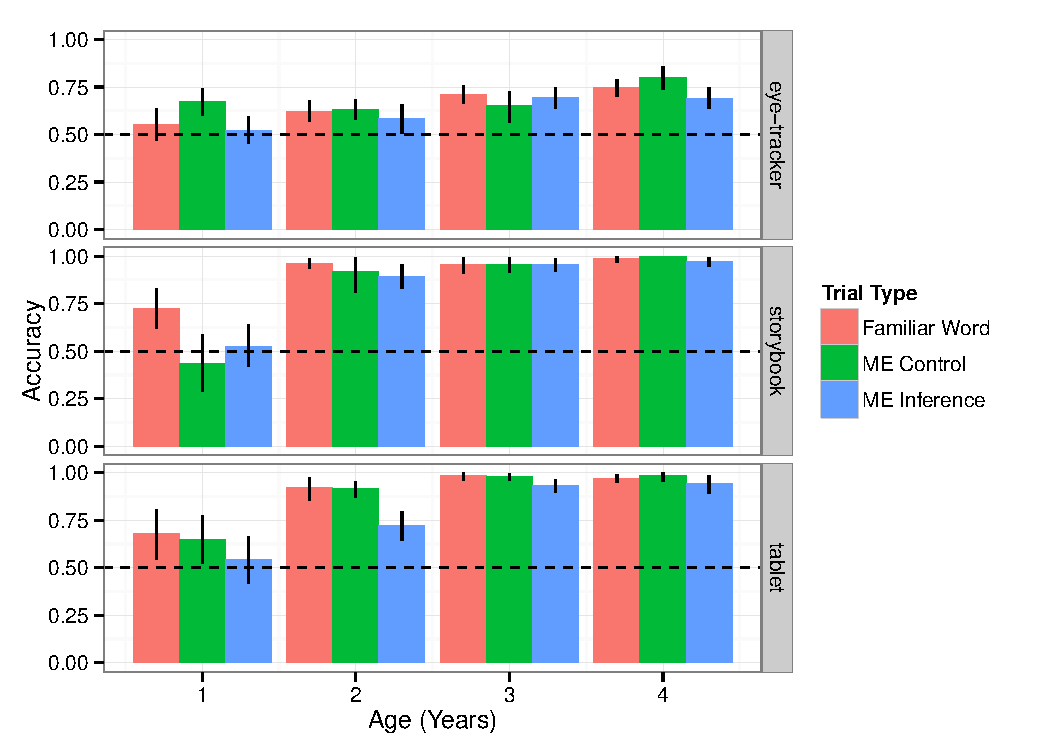
\includegraphics[width=5in]{figures/accuracy.pdf} 
    \caption{\label{fig:accuracy} Accuracy in our word recognition task, plotted by age group. Facets show different data collection modalities and trial types (ME refers to mutual exclusivity; see text for more details). Dashed line shows chance performance. Error bars show 95\% confidence intervals, computed by non-parametric bootstrap. }
  \end{center} 
\end{figure}

Word recognition accuracies across age groups and conditions are shown in Figure \ref{fig:accuracy} (see Appendix A for full details regarding this and subsequent analyses). Overall, older children (three- and four-year-olds) were close to ceiling in all trial types; but younger children's performance varied by both trial type and data collection condition. Data for the one-year-olds were the most variable: children were above chance for both Familiar Word and ME Control trials in the tablet condition, while for eye-tracker only ME control trials were above chance and for the storybook only Familiar Word trials were above chance. The tablet also revealed lower performance in the ME inference trials for the two-year-olds, in contrast with the other two methods. In sum, we found that accuracy data from the tablet revealed a sensible pattern of inferences---greater difficulty in ME inference trials than familiar word trials, combined with developmental change---and the tablet had at least the sensitivity of the comparison modalities. 

\subsubsection{Reaction time data}

\begin{figure}[t] 
  \begin{center} 
    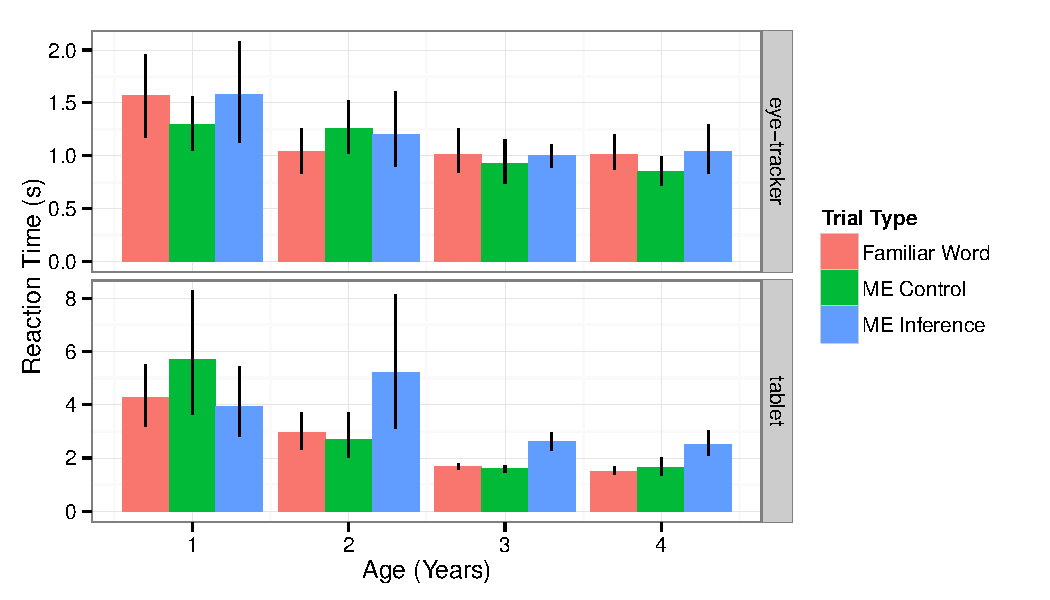
\includegraphics[width=5in]{figures/rt.pdf} 
    \caption{\label{fig:rt} Reaction times in our word recognition task, plotted by age group and trial type, with panels showing eye-tracker and tablet data (note different vertical scales). Error bars show 95\% confidence intervals, computed by non-parametric bootstrap.}
  \end{center} 
\end{figure}

Reaction times for the eye-tracker and tablet conditions are shown in Figure \ref{fig:rt}. While for both conditions, the primary trend was a decrease in reaction time for older children, several other patterns were also visible. First, reaction times for the tablet were several times longer than those for the eye-tracker, consistent with the more complex motor task of tapping a picture compared with making a saccade with the eyes. Second, the tablet but not the eye-tracker revealed slower reaction times for ME inference trials for the two-, three-, and four-year-olds, a pattern that had been observed in young children in a more age-specific and substantially longer eye-tracking paradigm \cite{bion2013}. 

One potential reason for the lack of sensitivity of the eye-tracking paradigm comes from the fact that two-alternative eye-tracking paradigms only yield reaction times for half of trials. No reaction time is computed on trials where the participant begins the trial looking at the target \cite{fernald2008}. In contrast, every trial on a tablet yields a reaction time; see Table \ref{tab:reliability} for the number of RT trials for each condition and age group. In sum, in a short paradigm of this type, the tablet was more successful in reproducing a previously-documented reaction-time effect.

\subsubsection{Reliability}

% latex table generated in R 3.1.1 by xtable 1.7-4 package
% Wed Feb 11 12:12:16 2015
\begin{table}[t]
\centering
\caption{\label{tab:reliability} Standardized Reliability Coefficients (Cronbach's $\alpha$)  for accuracy and reaction time by age group, along with the mean number of trials for each.}
\begin{tabular}{llcccc}
  \hline
Age & Condition & M Trials (acc) & $\alpha_{acc}$ & M Trials (RT) & $\alpha_{RT}$ \\ 
  \hline
1-year-olds & Eye-tracker & 7.65 & -0.98 & 4.47 & 0.88\\ 
    & Storybook & 13.00 & 0.77 & & \\ 
    & Tablet & 11.78 & 0.45 & 8.50 & 0.72\\ 
2-year-olds & Eye-tracker & 11.61 & 0.74 & 5.72 & 0.25 \\ 
    & Storybook & 13.00 & 0.69 & & \\ 
    & Tablet & 16.05 & 0.64 & 14.77 & 0.69\\ 
3-year-olds & Eye-tracker & 12.88 & 0.58 & 6.12 & 0.60\\ 
    & Storybook & 13.00 & 0.58 & & \\ 
    & Tablet & 15.83 & 0.06 & 15.54 & 0.59 \\ 
4-year-olds & Eye-tracker & 11.25 & 0.33  & 7.12 & 0.54 \\ 
    & Storybook & 13.00 & -0.11& &  \\ 
    & Tablet & 15.45 & 0.47 & 15.09 & 0.77 \\ 
   \hline
\end{tabular}
\end{table}

Group-level developmental differences above do not necessarily signal a measure with high reliability. To measure reliability differences directly, we computed Cronbach's $\alpha$, a standard statistic that quantifies the reliability of a set of measurements \cite{santos1999}. Our experiment contained eight trials from each trial type, a small number of trials on which to compute reliability statistics. So as to decrease data sparsity, we selected the 16 trials containing familiar words (both Familiar Word and ME Control trials) and computed a reliability coefficient for each age group and condition, for both reaction times and accuracies. Reliabilities are shown in Table \ref{tab:reliability}. 

Reliabilities were generally acceptable, with a few exceptions. First, the reliability of accuracies declined with age across conditions, because of ceiling effects: three- and four-year-olds made essentially no errors that distinguished between individuals. Second, the eye-tracker paradigm we used yielded only a limited amount of data for the youngest children. Because of the limited number of trials, reliability numbers for one-year-olds were noisy and we interpret these with caution. For two-year-olds, the age group for which this paradigm was most diagnostic (e.g., there were no floor or ceiling effects), the tablet yielded the best reliabilities. In sum, though there was substantial overall variability, the tablet was competitive in reliability with both eye-tracking and storybook methods. 

\section{Limitations of Tablets}

%While the evidence presented above suggests that tablets can be a powerful and flexible data collection modality for young children, there are nevertheless a number of limitations, both to our method and to the use of tablets more generally. 

The evidence presented above suggests that the tablet-based data collection replicates behavioral patterns observed in other modalities with comparable reliability for young children. There are nevertheless a number of limitations, both to our method and to the use of tablets more generally. 

% \subsection{Limitations of our method for data collection with tablets}

In our view, the specific web-based method we presented here has three primary limitations. First, it requires internet connectivity. For experiments in the field or in public places, this requirement may mean that other techniques are more appropriate. Second, it relies on a web-based development ecosystem that includes server-side technologies like PHP and client-side technologies including HTML, CSS, and JavaScript. While these open tools are well-documented and relatively easy to master, setting up these experiments still requires some technical orientation. If a lab is already hiring a programmer, it might be appropriate to build a native app rather than a web-based one. Third, there are cases where having a robust, native app might lead to better performance, especially when an experiment requires extensive media or animation, use of the tablet's camera, or large-scale data transfer.  For these reasons, data collection with a native app may be better suited for some projects.

% \subsection{Limitations of tablets more generally}

Tablets more generally also have a number of limitations that make them suitable for many but not all experiments. Below we consider three classes of limitations: participant variability in experience with tablets, limitations of measurement, and limitations associated with the novelty of the method.

\subsubsection{Limitations due to children's prior experience} 
Performance while interacting with a tablet depends to some degree  on children's prior experience with the tablet. Children who have prior experience may be better practiced at the motor skills necessary for indicating their responses. If children have not interacted with a tablet before, care must be taken to familiarize them with the device prior to data collection. There may also be population-level differences in experience with tablets, suggesting that researchers should exercise caution in cross-population comparisons of tablet-collected data.

\subsubsection{Limitations due to measurement issues} 
There are a number of limitations associated with measurement when using a tablet for data collection.  Reaction time measurements on the tablet appear reliable in the data we collected, but validation of the precision of reaction time recording will require more substantial technical efforts \cite<cf.>{crump2013}. In particular, it is likely that the precision of reaction times will vary somewhat from device to device, perhaps making tablets unsuited for paradigms which yield small time differences and which require very fast reactions. And although eye-tracking did not yield more reliable data in our comparison, it is likely that well-tailored eye-tracking experiments would eventually yield more reliable measurements, especially for younger children \cite{fernald2006}. Regardless of modality, the more closely an experiment is tailored to appropriate developmental population, the more likely it will be to yield interpretable data. 

\subsubsection{Limitations due to methodological novelty}
Because data collection with a tablet is a relatively new method, there are several limitations associated with its novelty. One issue is that the length or sophistication of the paradigms that can be implemented on tablets is still unknown. Another is related to  ethical concerns of electronic data collection. While storage and transmission of fully-anonymized data on our web server has been approved by our institutional review board, researchers should consult with their local IRBs to understand the issues that can arise in electronic data collection. We recommend that researchers never collect names or other identifying information in their tablet apps---instead, if such information is collected, it should be stored separately and more securely. Finally, tablet-based experiments in general require some technical expertise to implement (either as a web-based or native app) and hence can be slower for initial piloting than traditional behavioral methods. While these features of the tablet are limiting, they may be mitigated as tablet-based data collection becomes more widely used.

In sum, tablets are a powerful tool, but they are not suitable for every study; care should be taken to consider these limitations prior to beginning paradigm development. 


%Tablets more generally also have a number of limitations that make them suitable for many but not all data-collection opportunities. Below we list a number of limitations or qualifications on the use of this technology more broadly.



%
%\begin{itemize}
%\item If children have not interacted with a tablet before, care must be taken to familiarize children with the device prior to data collection. 
%\item Population-level comparisons of data collected with tablets may be problematic if the populations have differential levels of prior practice with tablets. 
%\item As when using other methods that yield reaction times, care must be taken in the analysis to establish a priori procedures for the detection and removal of outliers; otherwise, analyses will be subject to post-hoc bias based on data cleaning choices. 
%\item Tablet-based experiments require some technical expertise to implement (either as a web-based or native app) and hence can be slower for initial piloting than traditional behavioral methods. 
%\item The length or sophistication of the paradigms that can be implemented on tablets is still unknown and will require future work. 
%\item Although eye-tracking did not yield more reliable data in our comparison, for the youngest children, it is likely that well-tailored eye-tracking experiments will yield more reliable measurements \cite{fernald2006}. 
%\item Reaction time measurements on the tablet appear reliable in the data we collected, but validation of the precision of reaction time recording will require more substantial technical efforts \cite<cf.>{crump2013}. In particular, it is likely that the precision of reaction times will vary somewhat from device to device, perhaps making tablets unsuited for paradigms which yield small time differences and which require very fast reactions.
%\item While storage and transmission of fully-anonymized data on our web server has been approved by our institutional review board, researchers should consult with their local IRBs to understand the issues that can arise in electronic data collection. We recommend that researchers never collect names or other identifying information in their tablet apps---instead, such information should be stored separately and more securely if at all.
%\end{itemize}
%
%In sum, though tablets are a powerful tool, they are not suitable for every application; care should be taken to consider these limitations prior to beginning paradigm development. 

\section{Conclusions} 

We presented a simple method for creating tablet ``apps'' that allows experimenters to create basic websites and use these websites to collect data. This method is substantially easier and more flexible than tablet-native app development, which can be costly and time-consuming. In addition, our method allows cross-platform compatibility and easy sharing for the resulting experiments. We showed in a simple word recognition experiment that this method yields reliable reaction time and accuracy data for young children and compares favorably to two other standard data collection modalities. Data collection using tablets thus has the potential to supplement---and perhaps even supplant---many behavioral methods currently in use. 

Mobile and tablet-based computers are becoming increasingly commonplace in children's experience. Children play with their parents' and their own devices, and these devices are used for education, reading, games, and video chat with friends and relatives. Many important developmental issues are raised by this ubiquity, and more research must be done to determine how, when, and what children can learn from interactive media. Despite these issues, the opportunity posed by such devices for developmental psychologists is immense.


\bibliographystyle{apacite}
\bibliography{tablet}

\newpage

\theappendix

\section{Appendix A: Experimental Details}

\subsection{Methods}

\subsubsection{Participants}                                                                                                                              

  %    condition exclusion.crit  n
% 1  eye-tracker                71
% 2  eye-tracker   interference  4
% 3  eye-tracker           lang 25
% 4    storybook                73
% 5    storybook             dd  1
% 6    storybook   interference  4
% 7    storybook           lang 16
% 8    storybook  non-compliant  5
% 9       tablet                86
% 10      tablet             dd  1
% 11      tablet          error  2
% 12      tablet   interference  4
% 13      tablet           lang  7
% 14      tablet  non-compliant  1 + 1 (no data collected)

We recruited a sample of 228 one- to four-year-old children (1;0 -- 4;11) from the floor of Children's Discovery Museum of San Jose. Demographics for these participants are shown in Table \ref{tab:demo}. A first group of children was recruited for the tablet condition and then subsequently, children in the storybook and eye-tracker comparison groups were recruited and randomly assigned to one of these two conditions.

A number of additional children in the target age range were recruited but excluded from the sample for the following reasons: parent-reported English exposure less than our pre-specified criterion of 75\% (48), parent interference (12), non-compliance or difficulty with the experimental procedure (7), experimenter error or technical issues (2), and self-reported developmental disability (2). Parent interference was spread evenly across data collection conditions (4 in each). Of the non-compliant children, five were in the storybook condition, and two were in the tablet condition and could not complete the initial training phase.  

% latex table generated in R 3.1.1 by xtable 1.7-4 package
% Wed Feb 11 17:43:13 2015
\begin{table}[ht]
\centering
\caption{\label{tab:demo} Demographic information for the final sample of children in each data collection condition of our experiment.}
\begin{tabular}{lcccc}
  \hline
 Condition & Age Group & N & Mean Age & Prop. Male \\ 
  \hline
Tablet  & 1 &  18 & 1.71 & 0.44 \\ 
           & 2 &  22 & 2.46 & 0.68 \\ 
           & 3 &  24 & 3.56 & 0.67 \\ 
           & 4 &  22 & 4.51 & 0.59 \\  
Eye-tracker & 1 &  17 & 1.43 & 0.47 \\ 
           & 2 &  19 & 2.48 & 0.58 \\ 
           & 3 &  17 & 3.55 & 0.76 \\ 
           & 4 &  16 & 4.52 & 0.56 \\ 
Storybook & 1 &  15 & 1.62 & 0.60 \\ 
           & 2 &  19 & 2.49 & 0.32 \\ 
           & 3 &  19 & 3.48 & 0.53 \\ 
           & 4 &  20 & 4.48 & 0.45 \\ 
   \hline
\end{tabular}
\end{table}

\subsubsection{Stimuli}

Visual stimuli consisted of images of sixteen familiar and eight novel objects. All were presented as cropped images on a gray background with approximately the same resolution and detail.  Audio stimuli consisted of a carrier phrase (``Can you find the [target]?''), into which we spliced recordings of the target words. All recordings featured a female speaker and were created following the procedures described in \citeA{fernald2008}. We selected words from the MacArthur-Bates Communicative Development Inventory word list \cite{fenson1994,fenson2007}, choosing some words that we were certain nearly all children would be very familiar with (e.g., ``car,'' ``dog,'' ``bottle'') and others that were intended to be slightly more challenging (e.g., ``monkey,'' ``shovel,'' ``lion''). Novel words were mono- and di-syllabic words that had been used in previous experiments of this type (e.g. ``dax,'' ``pifo,'' ``kreeb''). We further included four fillers to break up the experiment (e.g., a picture of a child rowing a boat with a sentence describing it). All reaction times were computed from the onset of the target word. 

\subsubsection{Procedure}

Procedures were substantively identical in the three data-collection conditions. In each, experimental stimuli were presented in one of two pseudorandom lists, in which trials (pairs of pictures) were counterbalanced for order and target side. The three trial types were (1) \emph{Familiar Word} trials, in which two familiar pictures were presented and children were asked to select the image that matched a familiar word; (2) \emph{Mutual Exclusivity (ME) Control} trials, in which a familiar and a novel image were presented and children were asked to select the image that matched a familiar word; and (3) \emph{ME Inference} trials, in which a familiar and a novel image were presented and children were asked to select the image that matched a novel word. The experiment had 28 trials in total (eight of each of the three trial types plus four fillers). On each trial, two pictures were shown side-by-side as the sentence was presented.

Eye-tracking data were collected using an SMI RED 120Hz system. Children first completed a simple two-point calibration and then saw each trial presented on a static slide, accompanied by audio (played over speakers). Children were seated in a carseat mounted in an adjustable-height barber chair. 

The storybook was a three-ring binder containing printouts of the slides that participants viewed in the eye-tracking condition. An experimenter read the carrier phrases and target words from a script.

For tablet data collection, the procedure was identical to the eye-tracking condition, with the exception of a pre-training phase, which consisted of a task to help children learn to tap appropriately on the iPad. To advance past this training page, children needed to tap a set of five dots in random locations; each dot transformed into an ``X'' when tapped; a second page showed the same game with smiley faces. We found that this fun training sequence helped children select pictures effectively during the rest of the experiment. During test trials, touches were disabled until 300 ms after the onset of the target word. After the target was touched, the participant's choice was highlighted with a red border and further touches had no effect.  

\subsection{Results}

\subsubsection{Accuracy}

Accuracy for the eye-tracker was calculated as the proportion of total time in the trial that participants spent fixating the target in the period starting 300 ms after the onset of the target word, divided by the summed looking at the target and the distractor. The eye-tracker showed relatively limited sensitivity to the word recognition of the youngest children; neither familiar word recognition nor ME inference performance was above chance ($t(16) = 1.23,~p = 0.24$, and $t(11) = 0.52,~p = 0.62$; different degrees of freedom are due to missing data). In contrast, ME control trial performance was above chance ($t(12) = 4.49,~p < 0.001$). Two-year-olds and older children were reliably above chance for all trial types, with the exception of two-year-olds in the ME inference trials who trended towards above chance performance ($t(17) = 1.98,~p = 0.06$). Overall, our impression was that the sensitivity of our eye-tracking paradigm was limited relative to other experiments of this type \cite{fernald2006}, perhaps due to the necessity of designing a stimulus set that was relatively engaging for the full age range we studied. 

Accuracies were higher for the storybook and tablet conditions. In both conditions, responding was above chance for one-year-olds in familiar word trials (smallest $t > 2.57$, $p < .02$) and was above chance for the tablet in the ME control trials ($t(17) = 2.23,~p = 0.04$) but not for the other trial types. 

To equate across the slightly different age distributions for the different groups, and to quantify the broader pattern of differences, we fit a logistic mixed effects model to data from the tablet and storybook condition \cite{jaeger2008}. We specified fixed effects of age (continuous), condition, and trial type (dummy coded, with familiar word trials as the intercept) and all interactions, and with random effects of trial type varying by participant. We found significant main effects of age ($\beta = 1.17,~p < .0001$) and trial type (ME control, $\beta = -3.86,~p <.0001$, ME inference, $\beta = -1.36,~p = .05$). We also found significant age by trial type, condition by trial type, and age by condition by trial type interactions for the ME control trials, capturing the pattern that these trials were relatively more difficult for younger children in the storybook condition than the tablet condition.

\subsubsection{Reaction Time}

We did not measure reaction times (RTs) in the storybook condition; though coding these from video would in principle have been possible, timing was not tightly controlled. RTs on the tablet were defined as the time from word onset to first tap on correct trials. Eye-tracking RTs were defined as the time to switch from distractor to target on trials where the eyes were initially fixating the distractor at the point of disambiguation \cite<for more details, see>{fernald2008}. For the tablet RT data, we found a significant proportion of extreme outliers. In an exploratory analysis, we fit a Gaussian mixture model and found that the best BIC values were produced by a two-cluster solution---featuring a large faster cluster and a small, very slow cluster, probably interpretable as children who were hesitant to respond.

We excluded RTs faster than 500 ms or slower than 4000 ms. These values were determined post-hoc, based on visual inspection of the distribution. They correspond well both to our intuitions about the task and to our exploratory analyses (and resulted in a loss of 10.9\% of values). In future work, we recommend the adoption of {\it a priori} standards for RT exclusion; we did not do so here because exploring such standards was a goal of the current experiment. Experimenting with other reaction-time outlier exclusion processes did not qualitatively alter the pattern of results. Nevertheless, we recommend that investigators using this method carefully examine their distribution of reaction times, as averages can be heavily skewed by just a small number of very long RTs.

Overall, older children were faster in both the eye-tracker and tablet conditions. Because of the different magnitudes of RTs across the two conditions, we fit independent linear mixed effect models to the logarithm of reaction time for each. A model fit to the eye-tracker data revealed only a main effect of age. A model fit to the eye-tracker data with fixed effects of age (continuous), trial type, and their interaction and random effects of trial type by participant revealed only a highly reliable main effect of age. No further patterns were visible in the eye-tracker data, perhaps due to the relatively low number of trials that were included in this analysis. (Computing RTs from two-alternative eye-tracking data requires excluding approximately half of all trials, because the participant is already fixating the target at the point of disambiguation). In contrast, a model fit to the tablet data also showed a highly significant main effect of age ($\beta=-.24,~p < .0001$) and a significant age by trial type interaction such that ME inference trials were slower for older children ($\beta = 0.07,~p =.04$).

\end{document}
